\documentclass[10pt]{extarticle}
\title{}
\author{Avinash Iyer}
\date{}
\usepackage[shortlabels]{enumitem}

%font setup
%
%\usepackage{newpxtext,eulerpx}

%paper setup
\usepackage{geometry}
\geometry{letterpaper, portrait, margin=1in}
\usepackage{fancyhdr}

%symbols
\usepackage{amsmath}
\usepackage{amssymb}
\usepackage{mathtools}
\usepackage{hyperref}
\usepackage{gensymb}
\usepackage{multirow,array}

\usepackage[T1]{fontenc}
\usepackage[utf8]{inputenc}

%chemistry stuff
\usepackage[version=4]{mhchem}
\usepackage{chemfig}

%plotting
\usepackage{pgfplots}
\usepackage{tikz}
\tikzset{middleweight/.style={pos = 0.5, fill=white}}
\tikzset{weight/.style={pos = 0.5, fill = white}}
\tikzset{lateweight/.style={pos = 0.75, fill = white}}
\tikzset{earlyweight/.style={pos = 0.25, fill=white}}

%\usepackage{natbib}

%graphics stuff
\usepackage{graphicx}
\graphicspath{ {./images/} }

%code stuff
%when using minted, make sure to add the -shell-escape flag
%you can use lstlisting if you don't want to use minted
%\usepackage{minted}
%\usemintedstyle{pastie}
%\newminted[javacode]{java}{frame=lines,framesep=2mm,linenos=true,fontsize=\footnotesize,tabsize=3,autogobble,}
%\newminted[cppcode]{cpp}{frame=lines,framesep=2mm,linenos=true,fontsize=\footnotesize,tabsize=3,autogobble,}

%\usepackage{listings}
%\usepackage{color}
%\definecolor{dkgreen}{rgb}{0,0.6,0}
%\definecolor{gray}{rgb}{0.5,0.5,0.5}
%\definecolor{mauve}{rgb}{0.58,0,0.82}
%
%\lstset{frame=tb,
%	language=Java,
%	aboveskip=3mm,
%	belowskip=3mm,
%	showstringspaces=false,
%	columns=flexible,
%	basicstyle={\small\ttfamily},
%	numbers=none,
%	numberstyle=\tiny\color{gray},
%	keywordstyle=\color{blue},
%	commentstyle=\color{dkgreen},
%	stringstyle=\color{mauve},
%	breaklines=true,
%	breakatwhitespace=true,
%	tabsize=3
%}
% text + color boxes
\usepackage[most]{tcolorbox}
\tcbuselibrary{breakable}
\newtcolorbox{problem}[1]{colback = white, title = {#1}, breakable}
\newtcolorbox{solution}{colback = white, colframe = black!75!white, title = Solution, breakable}
%including PDFs
%\usepackage{pdfpages}
\setlength{\parindent}{0pt}

\pagestyle{fancy}
\fancyhf{}
\rhead{Avinash Iyer}
\lhead{Math 212: Homework 1}
\newcommand{\card}{\text{card}}
\newcommand{\ran}{\text{ran}}
\newcommand{\N}{\mathbb{N}}
\newcommand{\Q}{\mathbb{Q}}
\newcommand{\R}{\mathbb{R}}
\begin{document}
  \begin{problem}{12.1}
    \begin{itemize}
      \item 4: $B$ is closest to the $yz$ plane, lies on the $xz$ plane, and is farthest from the $xy$ plane.
      \item 8: I and IV lie on the graph of $z=4$.
      \item 12:
        \begin{center}
          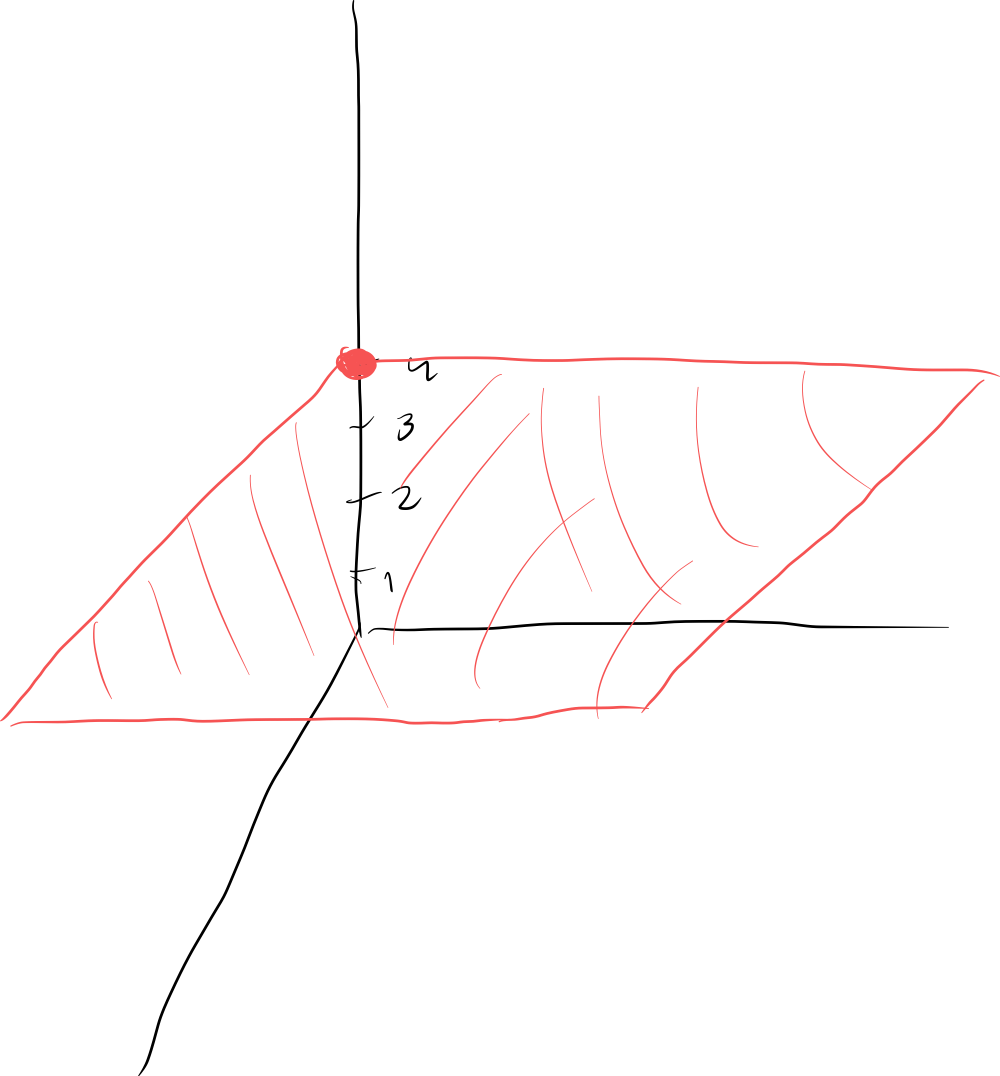
\includegraphics[width=10cm]{12_1_12}
        \end{center}
      \item 14:
        \begin{center}
          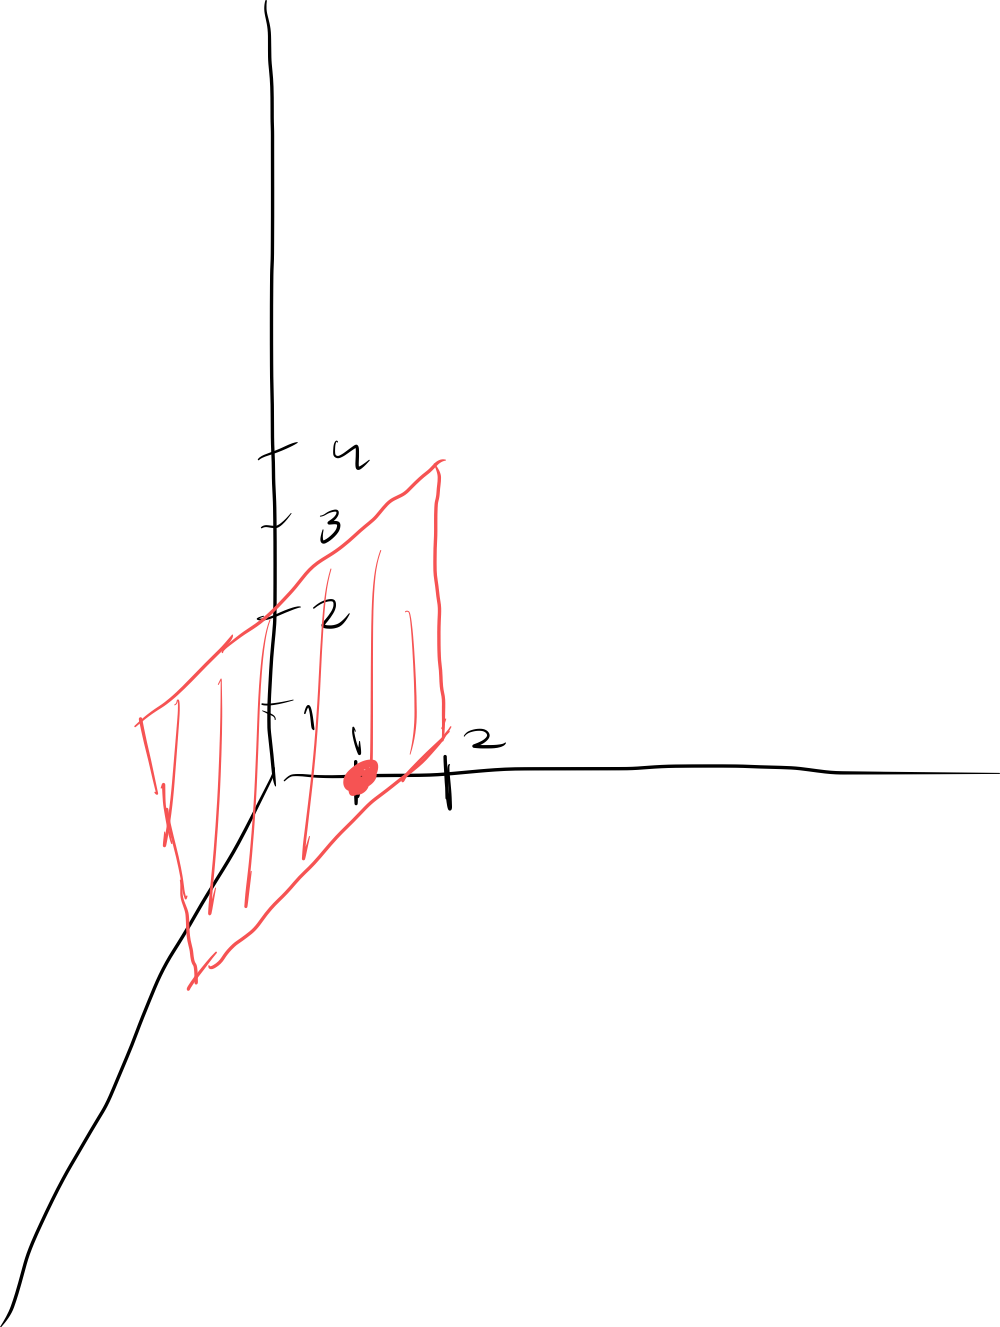
\includegraphics[width=10cm]{12_1_14}
        \end{center}
      \item 26:
        \begin{enumerate}[(a)]
          \item $-19^{\circ}$
          \item $20$ mph
          \item $17$ mph
          \item $16^{\circ}$
        \end{enumerate}
      \item 28:
        \begin{center}
          \renewcommand{\arraystretch}{1.5}
          \begin{tabular}{|c||c||c|c|c|c|c|c|c|c|}
            \hline
            \multicolumn{10}{|c|}{Temperature ($^{\circ}$F)}\\
            \hline
            \multirow{3}{7em}{Wind Speed (mph)}&& 35 & 30 & 25 & 20 & 15 & 10 & 5 & 0 \\
            \cline{3-10}
            & 5 & 31 & 25 & 19 & 13 & 7 & 1 & $-5$ & $-11$\\
                                               & 20 & 24 & 17 & 11 & 4 & $-2$ & $-9$ & $-15$ & $-22$\\
                                               \hline
          \end{tabular}
        \end{center}
        \item 32: $24.33$
        \item 34: $W\leq 46.2$ kg
        \item 38: Gravity acts on a $100$ kg mass at $7000$ km with approx. 820 newtons of force.
        \item 58: $(-1,-2,-7)$
    \end{itemize}
  \end{problem}
  \begin{problem}{12.2}
    \begin{itemize}
      \item 2: I, II
      \item 4: II, III
      \item 6:
        \begin{enumerate}[(a)]
          \item I
          \item V
          \item IV
          \item II
          \item III
        \end{enumerate}
      \item 24:
      \item 28:
        \begin{enumerate}[(a)]
          \item V
          \item IX
          \item VII
          \item I
          \item VIII
          \item II
          \item VI
          \item III
          \item IV
        \end{enumerate}
      \item 30:
      \item 32:
      \item 42:
    \end{itemize}
  \end{problem}
  \begin{problem}{12.3}
    \begin{itemize}
      \item 4: 
      \item 6:
      \item 8:
      \item 12:
      \item 16:
      \item 28:
      \item 36:
    \end{itemize}
  \end{problem}
\end{document}
